\documentclass[12pt,letterpaper]{article}
\usepackage[latin1]{inputenc}
\usepackage[spanish]{babel}
\usepackage{graphicx}
\usepackage[left=2cm,right=2cm,top=2cm,bottom=2cm]{geometry}
\usepackage{graphicx} % figuras
\usepackage{subfigure} % subfiguras
\usepackage{float} % para usar [H]
\usepackage{amsmath}
\usepackage{txfonts}
\usepackage{stackrel} 
\usepackage[latin1]{inputenc}
\usepackage{multirow}
\usepackage{enumerate} % enumerados
\renewcommand{\labelitemi}{$-$}
\renewcommand{\labelitemii}{$\cdot$}
\author{Nelia Escalante}
\title{Caratula}
\begin{document}

\title{Caratula}

\begin{titlepage}
\begin{center}
\large{UNIVERSIDAD PRIVADA DE TACNA}\\
\vspace*{-0.025in}
\begin{figure}[htb]
\begin{center}

\includegraphics[width=11cm]{./IMG/logo}
\end{center}
\end{figure}
\Large INGENIERIA DE SISTEMAS  \\

\vspace*{0.5in}
\begin{large}
\textbf{TITULO:} \\
\end{large}

\vspace*{0.1in}
\begin{Large}
\textbf{Creando un Reporte Interactivo en Power BI} \\
\end{Large}

\vspace*{0.3in}
\begin{Large}
\textbf{CURSO:} \\
\end{Large}

\vspace*{0.1in}
\begin{large}
INTELIGENCIA DE NEGOCIOS\\
\end{large}

\vspace*{0.3in}
\begin{Large}
\textbf{DOCENTE:} \\
\end{Large}

\vspace*{0.1in}
\begin{large}
 Ing. Patrick Cuadros Quiroga\\
\end{large}

\vspace*{0.2in}
\vspace*{0.1in}
\begin{large}
\textbf{ESTUDIANTE:} \\
\vspace{\baselineskip}
\begin{flushleft}

Escalante Maron, Nelia 		\hfill	(2014049551) \\

\end{flushleft}
\end{large}
\end{center}

\end{titlepage}

\newpage

	\begin{center}
		\Large Practica de Laboratorio 03
	\end{center}
	\vspace{\baselineskip}
	\vspace{\baselineskip}
	\textbf{\Large 1. RESULTADOS DEL DESARROLLO:}
	\\\\
Ejercicio 1: Conectando a Power BI a Datos \\\\

Tarea 1: Conectar a datos existentes\\\\ 
1. Abrir SQL Server Management Studio, y conectar a la instancia de base de datos (local) utilizando
autenticacion de Windows.\\\\ 
2. En el menú Archivo (File), en el submenu Abrir (Open), hacer click en Project/Solution, y buscar el archivo
Project.ssmssln.\\\\ 
3. En el Explorador de Soluciones, expandir Consultas (Queries), y luego hacer doble click en el archivo Lab
Exercise 1.sql.\\\\ 
\begin{center}
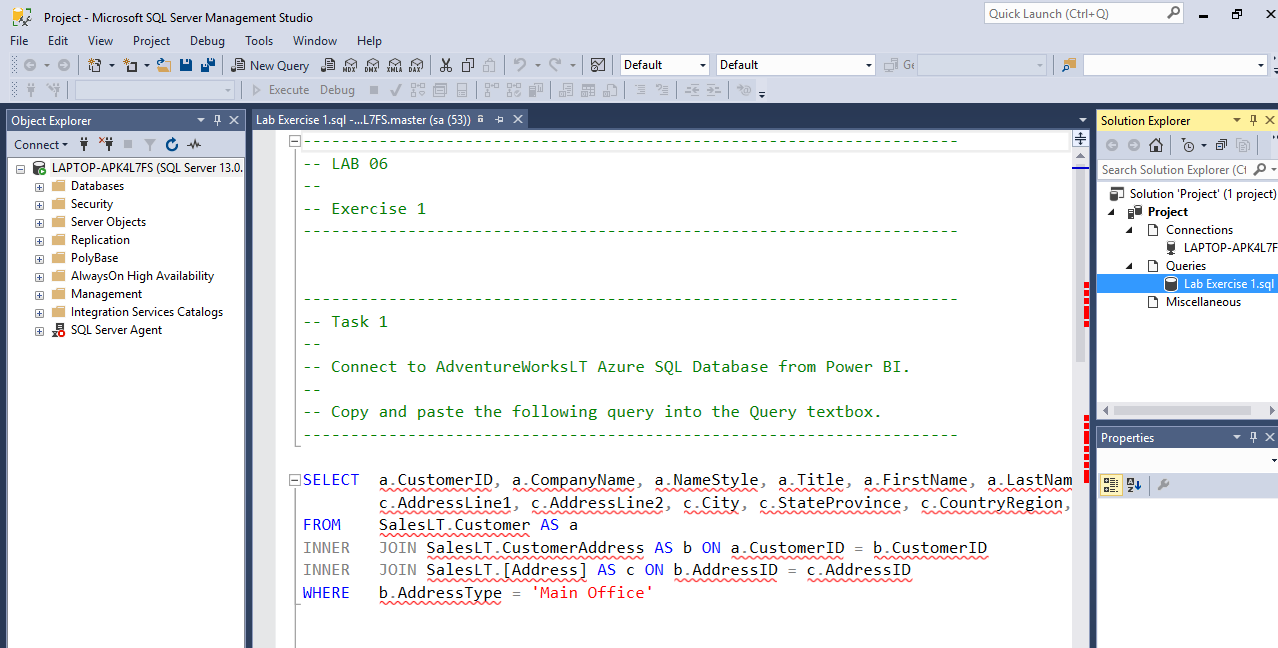
\includegraphics[width=9cm]{IMG/3.png} 
\end{center}
4. Abrir Power BI Desktop\\\\ 
5. In the Power BI Desktop window, click Get Data.\\\\
\begin{center}
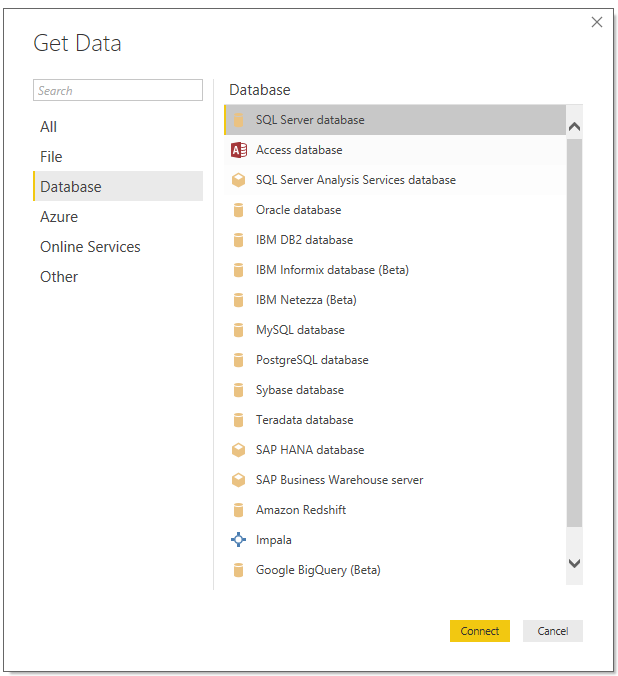
\includegraphics[width=9cm]{IMG/31.png} 
\end{center}
6. In the Get Data dialog box, click Microsoft SQL database, and then click Connect.\\\\
7. In the SQL Server database window, in the Server box, type (local).\\\\
8. In the Database (optional) box, type AdventureWorksLT.\\\\
9. Expand the Advanced options box.\\\\
10. In SQL Server Management Studio, copy the query under Task 1 in the Lab Exercise 1.sql query.\\\\
\begin{center}
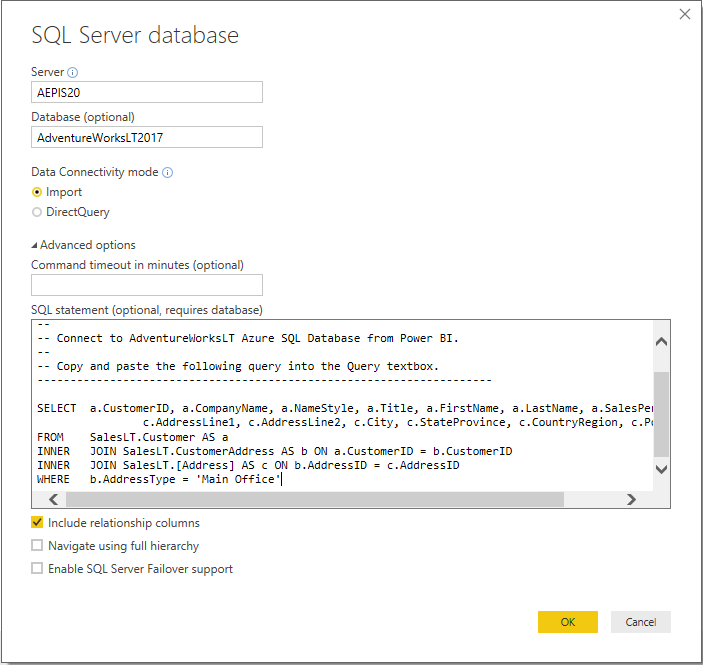
\includegraphics[width=9cm]{IMG/32.png} 
\end{center}
11. In Power BI Desktop, paste the query into the SQL statement (optional, requires database) box, and then click OK.\\\\
12. If the Access a SQL Server Database window appears. Click Connect.\\\\
13. In the data preview window, click Load.\\\\
\begin{center}
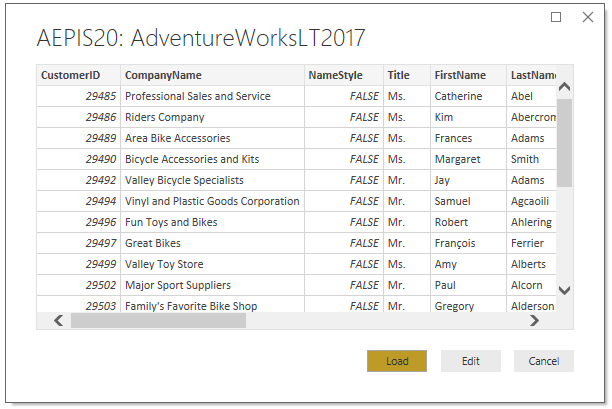
\includegraphics[width=9cm]{IMG/33.png} 
\end{center}
14. In Power BI Desktop, click Get Data then click More.\\\\
15. In the Get Data dialog box, click Microsoft SQL database, and then click Connect.\\\\
16. In the SQL Server database window, in the Server box, type (local).\\\\
17. In the Database (optional) box, type AdventureWorksLT.\\\\
18. Expand the Advanced options box.\\\\
19. In SQL Server Management Studio, copy the query under Task 2 in the Lab Exercise 1.sql query.\\\\
20. In Power BI Desktop, paste the query into the SQL statement (optional, requires database) box, and then click OK.\\\\
21. In the data preview window, click Load.\\\\
22. The window will close and return to the report, click Save.\\\\
23. In the Save As dialog box, in the File name box, type AdventureWorksLT Sales.pbix, and then click Save.\\\\
24. Leave Power BI Desktop open for the next task.\\\\

Task 2: Shape Data\\\\

1. In the Fields pane, right-click Query1, click Rename, type Customers, and then press Enter.\\\\
2. Right-click Query2, click Rename, type Sales, and then press Enter.\\\\
3. Expand the two tables to display all of the fields.\\\\
4. In the left navigation bar, click Data.\\\\
5. In the Fields pane, click the Customers table, if it is not already selected.\\\\
6. Right-click the NameStyle column, and click Delete.\\\\
7. In the Delete Column dialog box, click Delete.\\\\
\begin{center}
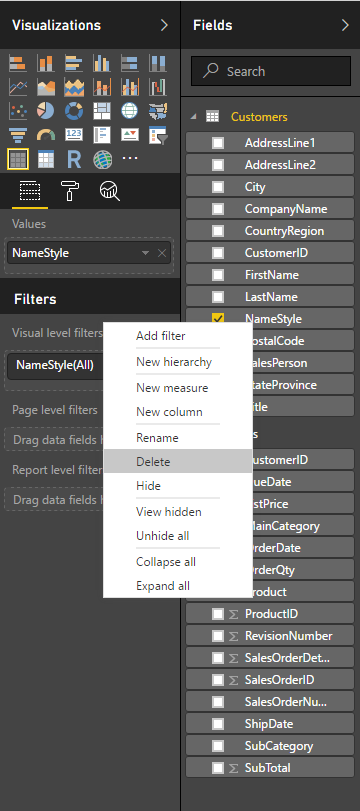
\includegraphics[width=5cm]{IMG/4.png} 
\end{center}
8. Right-click the SalesPerson column, and click Delete.\\\\
9. In the Delete Column dialog box, click Delete.\\\\
\begin{center}
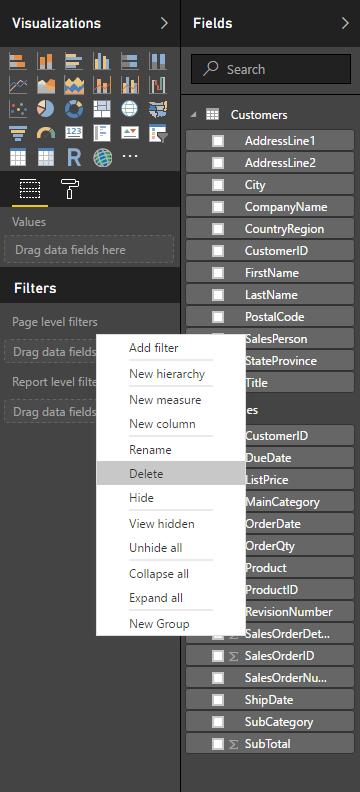
\includegraphics[width=4cm]{IMG/5.png} 
\end{center}
10. Right-click the CustomerID column, and then click Hide in Report View.\\\\
11. Click the AddressLine1 column header.\\\\
12. On the Modeling ribbon, in the Properties group, click Data Category: Uncategorized, and then click Address.\\\\
13. Click the City column header.\\\\
\begin{center}
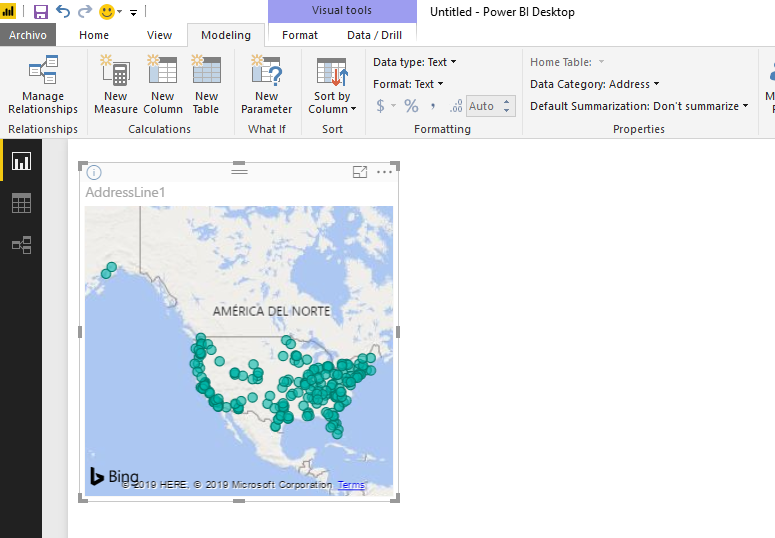
\includegraphics[width=9cm]{IMG/6.png} 
\end{center}
14. On the Modeling ribbon, in the Properties group, click Data Category: Uncategorized, and then click City.\\\\
15. Click the StateProvince column header.\\\\
\begin{center}
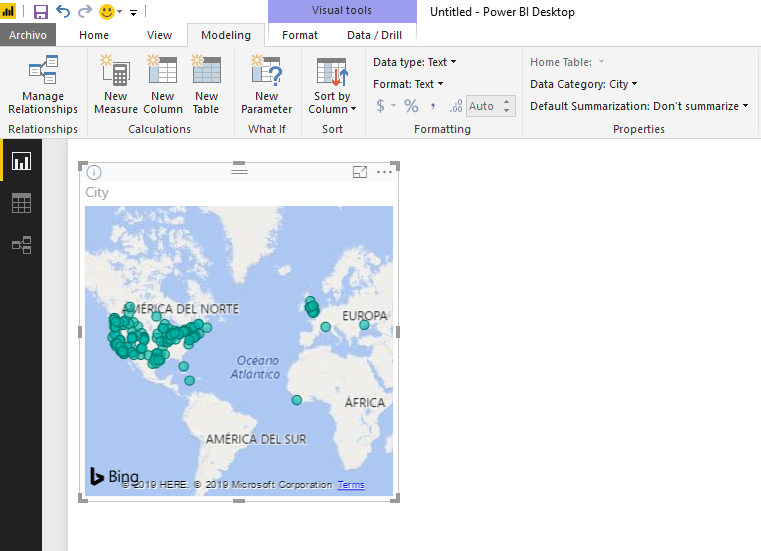
\includegraphics[width=9cm]{IMG/7.png} 
\end{center}
16. On the Modeling ribbon, in the Properties group, click Data Category: Uncategorized, and then click State or Province.\\\\
\begin{center}
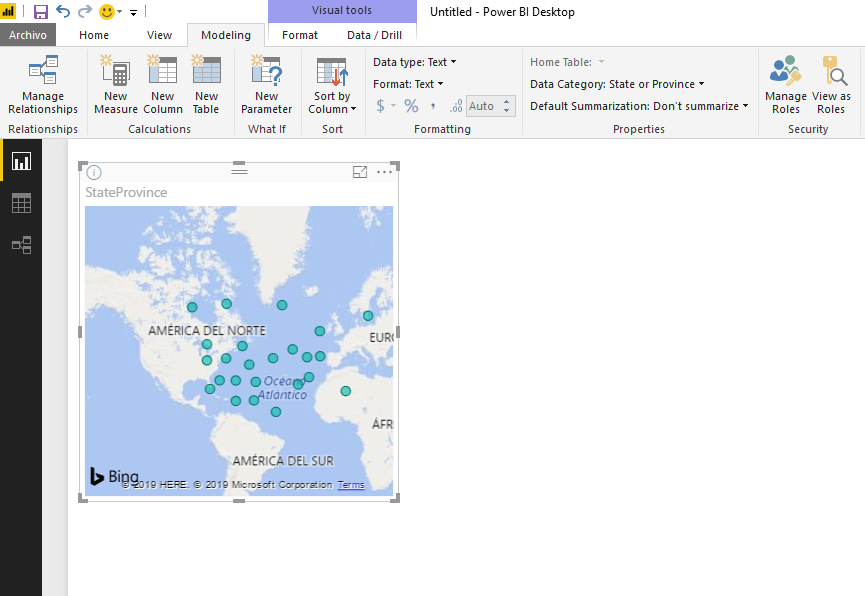
\includegraphics[width=9cm]{IMG/8.png} 
\end{center}
17. Click the CountryRegion column header.\\\\
18. On the Modeling ribbon, in the Properties group, click Data Category: Uncategorized, and then click Country/Region.\\\\
\begin{center}
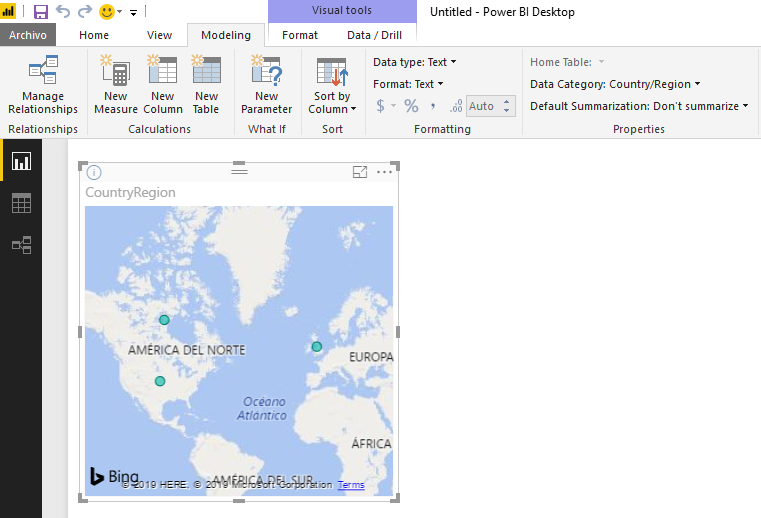
\includegraphics[width=9cm]{IMG/9.png} 
\end{center}
19. Click the PostalCode column header.\\\\
20. On the Modeling ribbon, in the Properties group, click Data Category: Uncategorized, and then click Postal Code.\\\\
\begin{center}
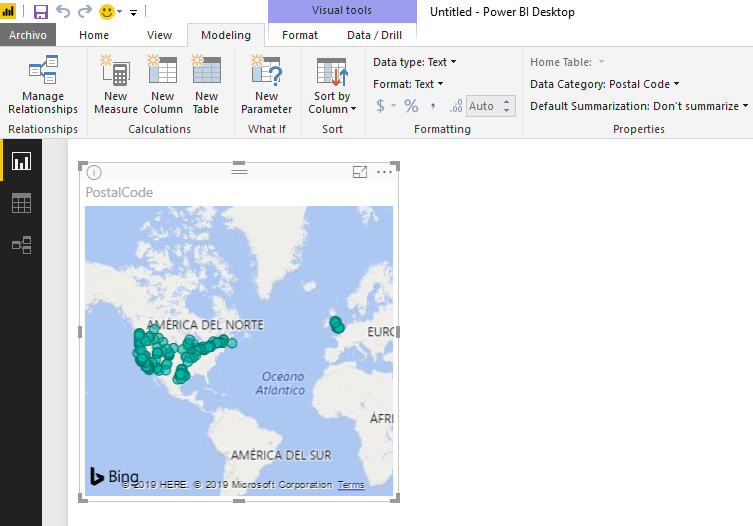
\includegraphics[width=9cm]{IMG/10.png} 
\end{center}
21. On the Modeling ribbon, in the Calculations group, click New Column, and then in the formula bar, type the following expression and press Enter:\\\\
\begin{center}
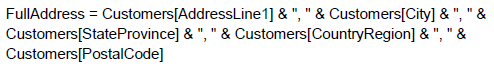
\includegraphics[width=9cm]{IMG/1.png} 
\end{center}
22. In the Fields pane, click Sales.\\\\
23. Right-click the RevisionNumber column, and click Delete.\\\\
24. In the Delete Column dialog box, click Delete.\\\\
25. Right-click the SalesOrderNumber column, and click Delete.\\\\
26. In the Delete Column dialog box, click Delete.\\\\
27. Right-click the CustomerID column, and then click Hide in Report View.\\\\
28. Right-click the SalesOrderID column, and then click Hide in Report View.\\\\
29. Right-click the SalesOrderDetailID column, and then click Hide in Report View.\\\\
30. On the Modeling ribbon, in the Calculations group, click New Column, and then in the formula bar, type the following expression and press Enter:\\\\

LineTotal = Sales[OrderQty] * Sales[ListPrice]\\\\
\begin{center}
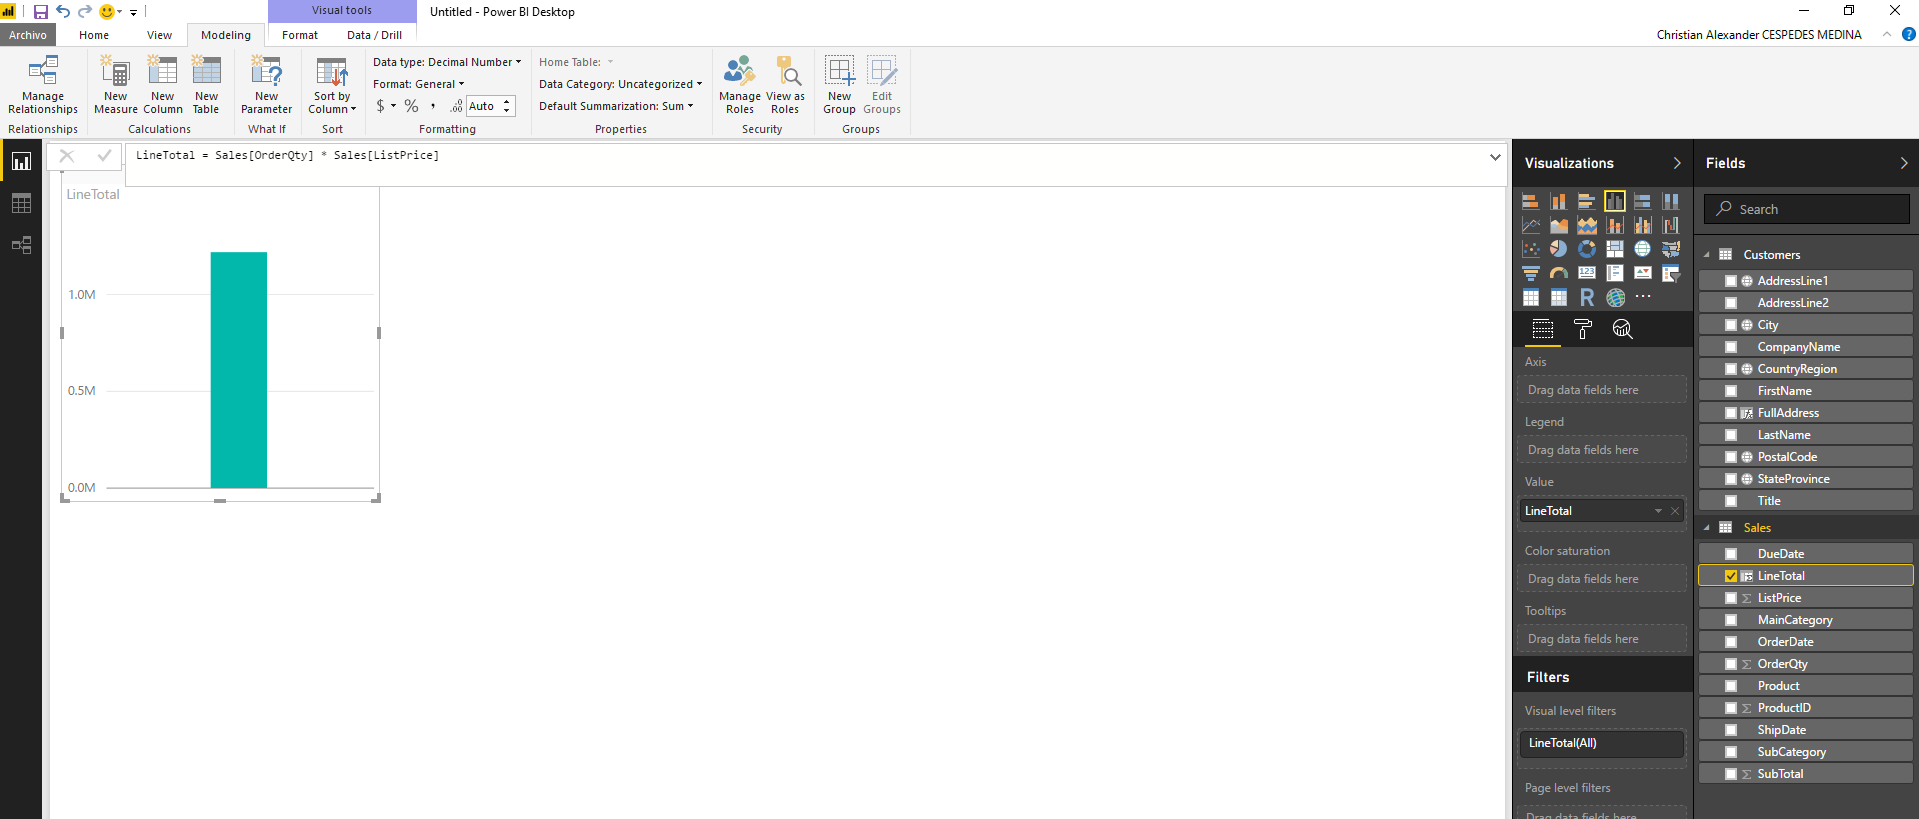
\includegraphics[width=9cm]{IMG/12.png} 
\end{center}
31. Click the LineTotal column header.\\\\
32. On the Modeling ribbon, in the Formatting group, click Format: General, point to Currency, and then click \$ English (United States).\\\\
33. On the Modeling ribbon, in the Calculations group, click New Measure, and then in the formula bar, type the following expression and press Enter.\\\\
TargetSales = SUM('Sales'[LineTotal]) * 1.2\\\\
\begin{center}
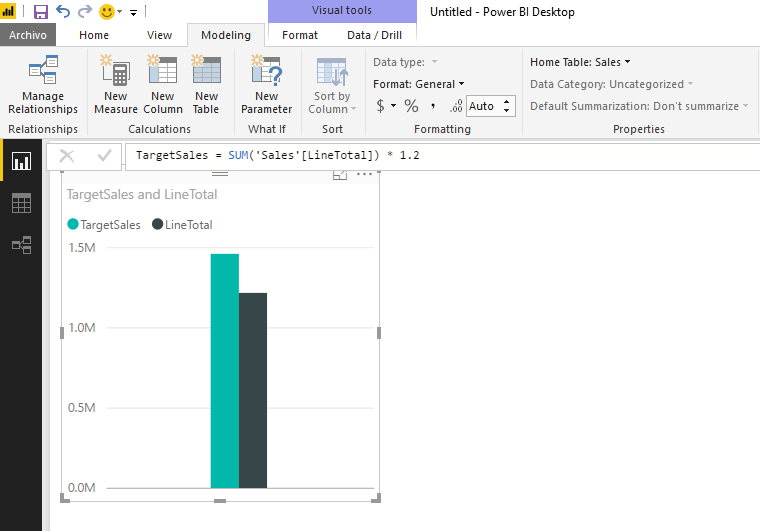
\includegraphics[width=9cm]{IMG/14.png} 
\end{center}
34. Click Save, and then leave Power BI Desktop open for the next task.\\\\



\end{document}